% This file was converted to LaTeX by Writer2LaTeX ver. 1.0.2
% see http://writer2latex.sourceforge.net for more info
\documentclass[a4paper]{article}
\usepackage[utf8]{inputenc}
\usepackage[T3,T1]{fontenc}
\usepackage[english]{babel}
\usepackage[noenc]{tipa}
\usepackage{tipx}
\usepackage[geometry,weather,misc,clock]{ifsym}
\usepackage{pifont}
\usepackage{eurosym}
\usepackage{amsmath}
\usepackage{wasysym}
\usepackage{amssymb,amsfonts,textcomp}
\usepackage{color}
\usepackage[top=2cm,bottom=2cm,left=2cm,right=2cm,includehead,head=12pt,headsep=0.499cm,includefoot,foot=12pt,footskip=26.144882pt]{geometry}
\usepackage{array}
\usepackage{supertabular}
\usepackage{hhline}
\usepackage{hyperref}
\hypersetup{pdftex, colorlinks=true, linkcolor=blue, citecolor=blue, filecolor=blue, urlcolor=blue, pdftitle=Master of Libre Software Vigo Edition, pdfauthor=José S.A., pdfsubject=Memory, pdfkeywords=memory; educational; software; libre; open source}
\usepackage[pdftex]{graphicx}
\makeatletter
\newcommand\arraybslash{\let\\\@arraycr}
\makeatother
% Footnote rule
\setlength{\skip\footins}{0.119cm}
\renewcommand\footnoterule{\vspace*{-0.018cm}\setlength\leftskip{0pt}\setlength\rightskip{0pt plus 1fil}\noindent\textcolor{black}{\rule{0.25\columnwidth}{0.018cm}}\vspace*{0.101cm}}
% Pages styles
\makeatletter
\newcommand\ps@Standard{
  \renewcommand\@oddhead{}
  \renewcommand\@evenhead{\@oddhead}
  \renewcommand\@oddfoot{\thepage{}}
  \renewcommand\@evenfoot{\@oddfoot}
  \renewcommand\thepage{\arabic{page}}
}
\newcommand\ps@FirstPage{
  \renewcommand\@oddhead{}
  \renewcommand\@evenhead{}
  \renewcommand\@oddfoot{}
  \renewcommand\@evenfoot{}
  \renewcommand\thepage{\arabic{page}}
}
\makeatother
\pagestyle{Standard}
\setlength\tabcolsep{1mm}
\renewcommand\arraystretch{1.3}
\title{Master of Libre Software Vigo Edition}
\author{José S.A.}
\date{2012-10-21}
\begin{document}
\clearpage\setcounter{page}{1}\pagestyle{Standard}
\thispagestyle{FirstPage}

\bigskip


\bigskip

{\centering
An Open Source Solution for Education Management
\par}

{\centering
EduXes
\par}


\bigskip


\bigskip


\bigskip


\bigskip


\bigskip

{\centering
\textit{José Antonio Salgueiro Aquino
{\textless}}\href{mailto:info@joseantonio.org}{\textit{info@joseantonio.org}}\textit{{\textgreater}
}
\par}

{\centering
\textit{Student of the V Master on Free Software Projects Development
and Management 2011-2012}
\par}

\clearpage{\itshape
Copyright (cc) 2012 José Antonio Salgueiro Aquino. Some rights reserved.
This work is free and is licensed under the conditions of Creative
Commons Attribution – Share Alike 3.0 Unsupported license. You can use,
distribute and reuse this work if the same license is applied and the
author is quoted}

\textit{Full text of the license can be read on
}\url{http://creativecommons.org/licenses/by-sa/3.0/deed.en}

{\centering \par}

\begin{figure}
\centering

\includegraphics[width=2.528cm,height=0.891cm]{PhoneGapProjectMSWLMemory-img/PhoneGapProjectMSWLMemory-img1.png}
\end{figure}
\setcounter{tocdepth}{10}
\renewcommand\contentsname{Contents}
\tableofcontents

\bigskip

\clearpage\section[Description of the practicum ]{Description of the
practicum }
\hypertarget{RefHeading114141570052158}{}Name: José Antonio Salgueiro
Aquino

Birth date: 5 august 1970

Education: B.Sc. in Fundamental Physics, University of Santiago de
Compostela University 1988-1993.

Current address: Marin (Pontevedra)

Current job: Secondary School teacher in Technology.

I have done on my spare time at home a management application for high
school teachers.

Working times (planned): 300 hours.

\ \ From 6th August, to 30 September, on an eight hours day basis.

This application involves several technologies:

\begin{itemize}
\item Java language.
\item Android skeleton application.
\item PhoneGap framework to develop multi-platform applications.
\item JQuery and JqueryMobile \ to develop mobile oriented applications.
\item JavaScript with Web Databases.
\item Git for version control system.
\end{itemize}
Meetings:

\ \ One meeting on August: Technologies to be used were stated, work
methodologies, first application windows (pages), Android version to be
used (2.3.3) because is the most popular. 

\ \ Several emails and \textit{gtalk} conversations about organization,
general problems were written.

Teleworking is done. 

Materials and special equipment used:

\ \ My own computer for main development: 

Hardware: Intel Quad, 6GiB RAM, 500GiB HD. 

Software: Debian Linux Wheezy (testing), Eclipse Juno, JQuery 1.8.1,
jQueryMobile 1.1.1, and PhoneGap-Cordova 1.8.1, Android Virtual Manager
2.3.3, Git 1.7.10.4-1.

For testing Sony-Ericsson Xperia V mobile phone, with USB cable.


\bigskip

\ \ \ \ \ \ \ \ %
%This is a short introduction (not longer than 5 pages), with at least the following information (when applicable), and any \ \ \ other relevant information you may consider:
%\ \ \ \ \ \ \ \ Your personal data
%\ \ \ \ \ \ \ \ Data of your tutor in the company that hosts your practicum
%\ \ \ \ \ \ \ \ Description of the company that hosts your practicum
%\ \ \ \ \ \ \ \ Description of the practicum offer (the original or a renewed \ \ \ one)
%\ \ \ \ \ \ \ \ Duration and dates
%\ \ \ \ \ \ \ \ Info related to the daily basis of the work
%\ \ \ \ \ \ \ \ \ \ \ \ \ \ \ \ {}- Telework or on{}-site
%\ \ \ \ \ \ \ \ \ \ \ \ \ \ \ \ {}- Working times
%\ \ \ \ \ \ \ \ \ \ \ \ \ \ \ \ {}- Location
%\ \ \ \ \ \ \ \ \ \ \ \ \ \ \ {}- Record (as in minutes or notes) of meetings or important communications
%\ \ \ \ \ \ \ \ Materials and special equipment used
%\ \ \ \ \ \ \ \ Technologies involved



\bigskip

\section{}
\clearpage\section[Work plan]{Work plan}
\hypertarget{RefHeading114161570052158}{}\subsection[Description and
objectives:]{Description and objectives:}
\hypertarget{RefHeading115461570052158}{}\ \ A multi-platform management
application for high school teachers is developed. It can be run on a
smart-phone or tablet, or even a personal computer. 

\ \ The actual objectives of the applications are
student{\textquotesingle}s management:

\begin{itemize}
\item \begin{itemize}
\item Attendance control.
\item Misbehaviour control.
\item Activities evaluation.
\end{itemize}
\end{itemize}
\ \ Application should include this features:

\begin{itemize}
\item \begin{itemize}
\item Data visualization. As table-like.
\item Server synchronization with a custom application or
Xade\footnote{Xade is the web application used to management by
educational community: teacher{\textquotesingle}s, headmasters,
administrative staff.}.
\end{itemize}
\end{itemize}
\ \ The final goal is to develop an application to make
teacher{\textquotesingle}s work easier and comfortable. Also an
objective is to write extensible code, which allow another developers
to take part into application development.

Tasks:

\ \ The current list of tasks are:

\begin{enumerate}
\item Study state-of-art solutions. 

\begin{enumerate}
\item Find out other solutions: PDAs and smart-phone or tablet related
and web-based applications.
\item Download to study and reuse graphical user interfaces, code or/and
database structure. 
\end{enumerate}
\item Develop database structure: tables and relationships. 
\item Preparation of development:

\begin{enumerate}
\item Build development environment: install Eclipse, Android Virtual
Machine, Aptana Plugin, JQuery, JQueryMobile and Phonegap.
\item Choose application name and folder{\textquotesingle}s policy.
\item Make a simple application: only a blank page.
\item Upload simple application into a git
repository\footnote{\ \ \url{https://github.com/joseantoniosa/EduXes/}}
\end{enumerate}
\item Development:

\begin{enumerate}
\item Populate database with sample data.
\item Groups:

\begin{itemize}
\item Make list of groups window.
\item Groups management window.
\end{itemize}
\item Students:

\begin{itemize}
\item Make list of students window.
\item Students management window (insert-update-delete students)
\end{itemize}
\item Timetable for actual date: list of groups for each day.
\item Add attendance, misbehaviour for each student.
\item Add error handling.
\item Retrieve and insert data from and to database
\item List of attendance, misbehaviour incidents.
\item Add activities grades for each student.
\item List students marks and final mark.
\item Activities management window (add-update-remove activities)
\item Management of student notes.
\item List of student notes. 
\end{enumerate}
\item Test into real hardware: Android 2.3.3 mobile phone.
\item Save or download data from database to disk.
\item Xade web interface.

\begin{enumerate}
\item Study Xade web interface.
\item Develop an ad-hoc application for retrieve Xade{\textquotesingle}s
data. 
\end{enumerate}
\item Develop an ad-hoc application for store data. 
\item Synchronization with a custom server or with Xade.
\item Test units.
\item User documentation. Manual with images.
\item Developer{\textquotesingle}s documentation.
\item Find out a website to host a forum, a bug report system,
\ documentation and application download.

In the following table a broad estimation of time spent in each task are
shown. \ 
\end{enumerate}

\bigskip

\begin{flushleft}
\tablehead{\hline
\centering \bfseries Tasks &
\centering\arraybslash \bfseries Time \ (hours)\\\hline}
\begin{supertabular}{|m{12.791cm}|m{3.8219998cm}|}
State-of-art solutions &
\centering\arraybslash 10\\\hline
Develop database &
\centering\arraybslash 8\\\hline
Preparation for development &
\centering\arraybslash 40\\\hline
Development. &
~
\\\hline
\ \ Populate database with sample data. &
\centering\arraybslash 20\\\hline
\ \ Groups. List and management &
\centering\arraybslash 50\\\hline
\ \ Students. List and management &
\centering\arraybslash 30\\\hline
\ \ Timetable for actual date &
\centering\arraybslash 80\\\hline
\ \ Add attendance, behaviour &
\centering\arraybslash 50\\\hline
\ \ Add error handling &
\centering\arraybslash 2\\\hline
\ \ Retrieve and insert data from and to database &
\centering\arraybslash 30\\\hline
\ \ List of attendance, misbehaviour incidents. &
\centering\arraybslash 12\\\hline
\ \ Add activities grades for each student. &
\centering\arraybslash 12\\\hline
\ \ List students marks and final mark. &
\centering\arraybslash 14\\\hline
\ \ Activities management window  &
\centering\arraybslash 14\\\hline
\ \ Management of student notes. &
\centering\arraybslash 20\\\hline
\ \ List of student notes.  &
\centering\arraybslash 2\\\hline
Test into real hardware &
\centering\arraybslash 20\label{ref:Estimated}\\\hline
Save data into disk &
\centering\arraybslash 10\footnotemark{}\\\hline
\bfseries\itshape Total &
\centering\arraybslash \bfseries\itshape 394\\\hline
\end{supertabular}
\end{flushleft}
\footnotetext{Estimated}

\bigskip

Motivation:

\ \ I am a Technologies teacher, in my daily work I have to evaluate
students work such as working with tools, cooperative work, cooperative
work with other classmates etc., besides usual activities as written
exercises. It could used a long sheet, or an awkward long spreadsheet,
but a portable device with a custom application should be desirable.

\ \ This application increases teacher{\textquotesingle}s productivity
because teacher only has to write attendance, or unpunctuality two
times (on official report and on application{\textquotesingle}s
window), and classroom notes and activity grades on very easy way.

\ \ The most important feature is to be as easy, fast and intuitive as
possible. It could be desirable to be platform independent (Android,
iOS, Windows RT), but Android is preferred because it is open source,
has a high market share, and to buy an Apple Macintosh computer is not
mandatory.

\ \ I wish to learn from this application how to develop a mobile
application, and several technologies: JQuery, \ jQueryMobile,
PhoneGap/Cordova, SQLITE, git repository management.


\bigskip

\subsection[Methodology:]{Methodology:}
\hypertarget{RefHeading115481570052158}{}\ \ This work was carried on
building little blocks, also called pages, and make up it into final
application. Database structure was separated from interface, and
interface was also separated into dynamic and static. Each new
functionality was written, tested, and polished. Each new function was
written from previous one, and son on.

\ \ Tools involved were Eclipse IDE (with plug-ins) and Android Virtual
Manager (AVM) on Debian GNU/Linux Wheezy. When a new functionality was
developed, application was tested on AVM, \ if it worked, source code
was polished, applicable was tested again, if it was satisfactory a new
change was committed into git repository. 

\subsubsection[Work plan:]{Work plan:}
\hypertarget{RefHeading149931801272074}{}
\bigskip

Several problems were faced:

\begin{itemize}
\item Eclipse environment: A stable, reliable and up-to-date IDE, with
several plug-ins is needed. Download vanilla Eclipse Juno from its
web-site is chosen because it is more stable, reliable, compatible with
newer versions. \ Aptana Javascript plugin was chosen because Aptana
allows source code auto-completion in JQuery.
\item PhoneGap and Android incompatibilities. Android 2.3.3 requires
JQuery-1.8.1 and does not work on higher versions. 
\item Error handlers. I have had several problems with
\textit{tx.executeSql(...)} function, it confused me with
\textit{db.transaction(...): }

{\itshape
tx.executeSql(sql, [parameters], \ successHandler, errorHandler)}

and

{\itshape
db.transaction(queryFunction, errorHandler, successHandler) \ }

have up to four and three parameters respectively, only first one is
mandatory. I rather use success and error handlers for
\textit{tx.executeSql} function, atomic error control could be better
choice.
\item Passing variables to functions: Only if another solution is not
known or feasible, global variables are used: named after
\textit{global\_*}, and in block capitals.
\item Deadline. Development was delayed because I have no enough spare
time and above problems were time costly.
\end{itemize}
\section{}
\clearpage\section[Results]{Results}
\hypertarget{RefHeading114181570052158}{}Application is evolving from
list, edit students and groups, to its final goals. These objectives
were fulfilled:

\begin{itemize}
\item \begin{itemize}
\item Access to any workday, any group and student.
\item Management of attendance and misbehaviour of each student. The
students information is still hard-coded into source files.
\end{itemize}
\end{itemize}
There are obvious and easy to reach objectives:

\begin{itemize}
\item \begin{itemize}
\item Links to student and group management. These pages were done but
links are not missing into main application window.
\end{itemize}
\end{itemize}
There are several objectives not fulfilled yet, but I am on the way to
get those done, those are, in priority order:

\begin{itemize}
\item \begin{itemize}
\item Data visualization. Student attendance and misbehaviour have to be
shown in table-like window.
\item Test into real hardware. \textit{EduXes.apk} has to be copied into
mobile phone.
\item Activities evaluation per student. A window to display activities
marks and final mark.
\item Timetable management. A window to manage groups timetable. When a
group has class with this teacher.
\item Server synchronization with a custom application or
\end{itemize}
\end{itemize}
These objectives were not fulfilled because time and skills lack.

\clearpage
\bigskip

\subsection[Tasks completed]{Tasks completed}
\hypertarget{RefHeading115501570052158}{}\subsubsection[State{}-of{}-art
solutions]{State-of-art solutions}
\hypertarget{RefHeading146461801272074}{}\ \ Only an open source
application was found for study,
Siestta\footnote{\ \url{http://siestta.sourceforge.net/}},
\ nevertheless there are a lot of educational software
(Sixa\footnote{\ \url{http://www.sixa.es/es}},
Unisoft\footnote{\ \url{http://www.unisoftcolombia.com/unisoftcolombia/index.php}})
but they are privative, Microsoft Windows freeware or both (SAS
académico\footnote{\url{http://www.rafaelvarela.com/sas-academico-software-notas-boletines-matriculas.html}}).


\ \ Siestta was evaluated. 

Technically it is an GPL{\textquotesingle}ed old style PHP-based web
application with Ajax, an interactive editor, fckeditor and fpdf to
generate reports.

From user point-of-view there are online
documentation\footnote{\url{http://siestta.sourceforge.net/doc/index.html}}.
This application includes management of students, attendance, marks,
tasks, incidents, general queries, letters to parents, interviews with
parents, messages, appointments, exams and more.

\ \ Several screen-shots were taken and will be reused in current
application:



\begin{figure}
\centering
\begin{minipage}{17cm}

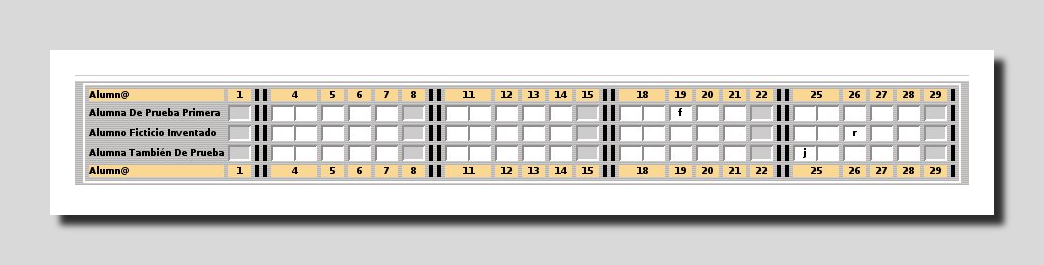
\includegraphics[width=17cm,height=4.314cm]{PhoneGapProjectMSWLMemory-img/PhoneGapProjectMSWLMemory-img2.png}
\caption[Attendance list. (From Siestta webpage)]{Attendance list. (From
Siestta webpage)}
\end{minipage}
\end{figure}


\begin{figure}
\centering
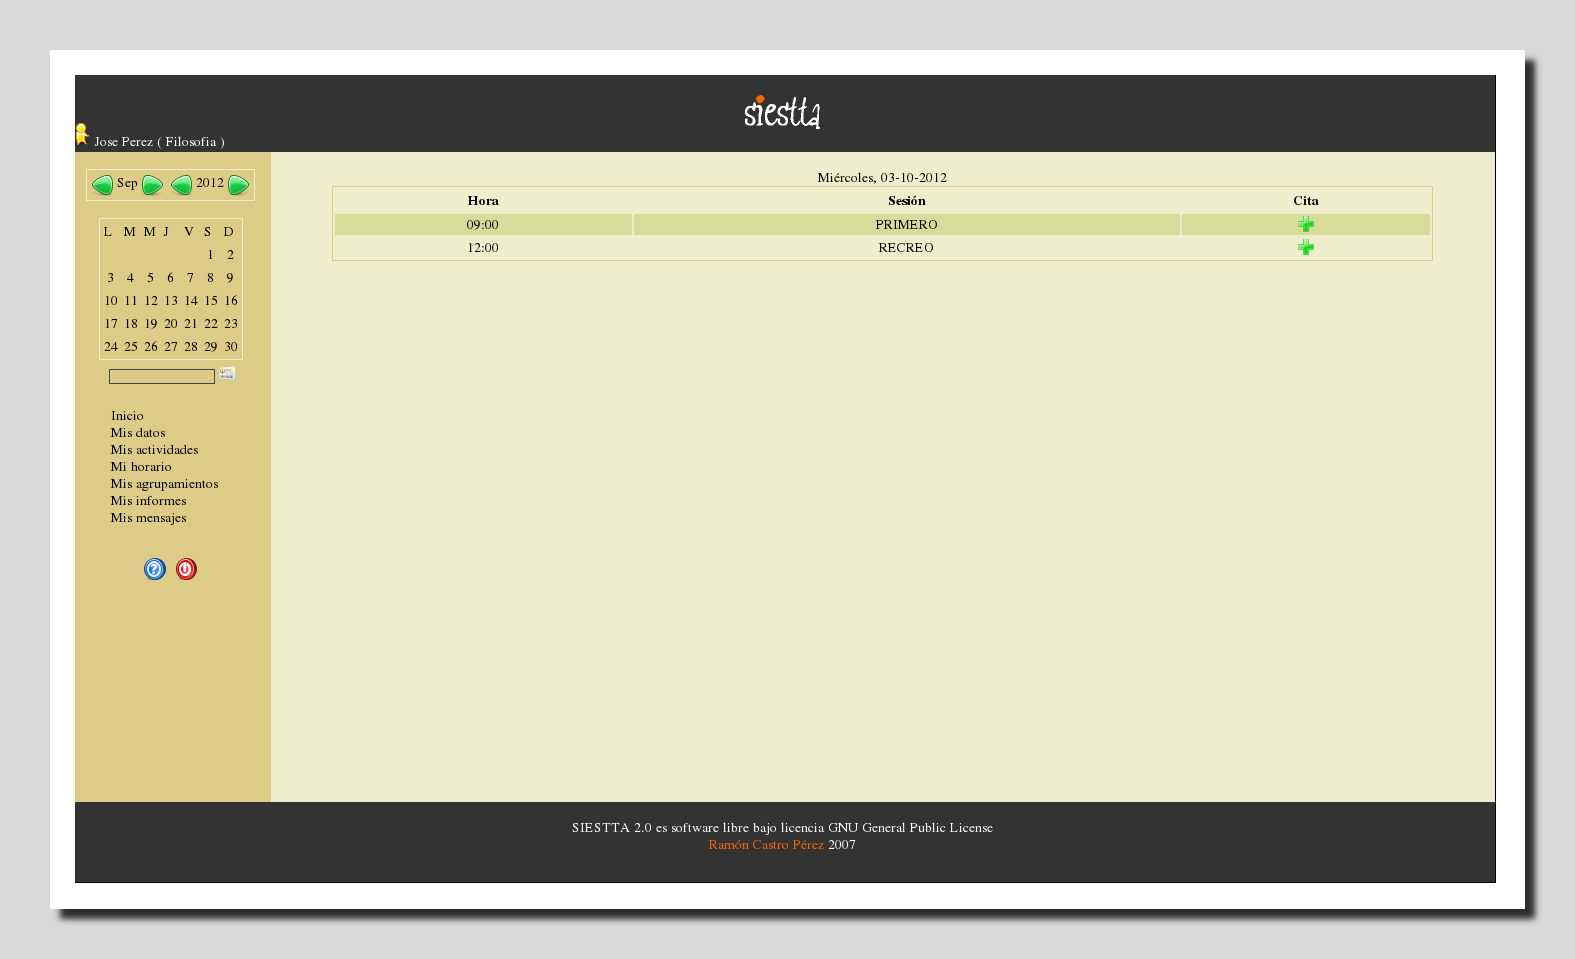
\includegraphics[width=17cm,height=10.351cm]{PhoneGapProjectMSWLMemory-img/PhoneGapProjectMSWLMemory-img3.png}
\caption[Main window (From local installation)]{Main window (From local
installation)}

\end{figure}


\begin{figure}
\centering
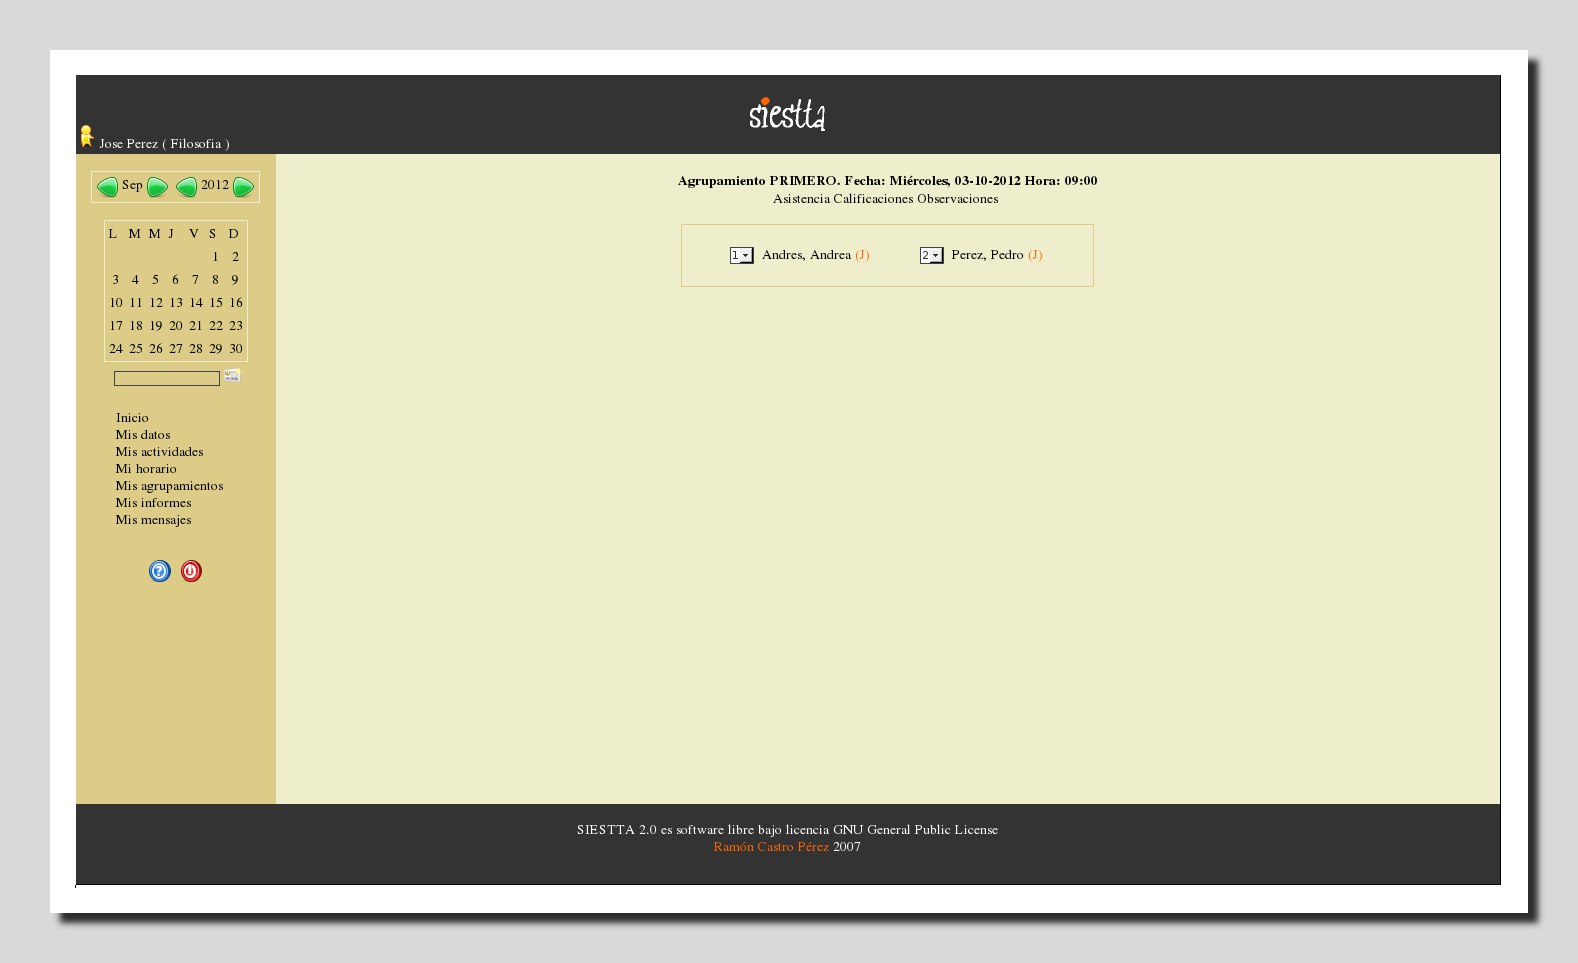
\includegraphics[width=17cm,height=10.373cm]{PhoneGapProjectMSWLMemory-img/PhoneGapProjectMSWLMemory-img4.png}
\caption[Attendance (From Siestta local installation)]{Attendance (From
Siestta local installation)}

\end{figure}
This application (Siestta) are also available for PDAs, it could be a
valid solution but it is server-side with outdated technologies. Data
structure from Siestta is standard and fully functional, and it could
be partially reused by EduXes.

\begin{figure}
\centering
 [Warning: Image ignored] % Unhandled or unsupported graphics:
%\includegraphics[width=17cm,height=23.823cm]{PhoneGapProjectMSWLMemory-img/PhoneGapProjectMSWLMemory-img5}
\caption[Siestta database structure.]{Siestta database structure.}

\end{figure}
Source code are also shown: \textit{calendario.php}. It shows us a PHP
application which uses sessions variables and is not
Model-View-Controller oriented.

\begin{enumerate}
\item[] 
\bigskip
\end{enumerate}
{\textless}?php 

session\_start(); 

require({\textquotesingle}config.php{\textquotesingle}); 

require({\textquotesingle}idioma/{\textquotesingle}.\$idioma.{\textquotesingle}{\textquotesingle});


include({\textquotesingle}funciones\_calendario.php{\textquotesingle}); 

\$docente =
\$\_SESSION[{\textquotesingle}usuario\_sesion{\textquotesingle}]; 

//recogemos variables 

\$mes\_actual = \$\_POST[{\textquotesingle}mes{\textquotesingle}]; 

\$anyo\_actual = \$\_POST[{\textquotesingle}anyo{\textquotesingle}]; 

if(\$mes\_actual {\textbar}{\textbar} \$anyo\_actual) \{ 

\ \ include({\textquotesingle}funciones.php{\textquotesingle}); 

\ \ conecta(); 

\ \ \} 

//si es la primera vez que entramos, cargamos la fecha actual 

if(!isset(\$mes\_actual)) \$mes\_actual =
date({\textquotesingle}m{\textquotesingle}); 

if(!isset(\$anyo\_actual)) \$anyo\_actual =
date({\textquotesingle}Y{\textquotesingle}); 

//presentamos ahora el calendario del mes actual o cargado 

//tabla con nombre mes y año y las flechas para navegar 

echo {\textquotesingle} 

{\textless}br /{\textgreater} 

{\textless}table
class={\textquotedbl}tablacentrada\_i{\textquotedbl}{\textgreater} 

{\textless}tr{\textgreater} 

{\textless}td{\textgreater} 

{\textless}a href={\textquotedbl}\#{\textquotedbl}
onclick={\textquotedbl}navegaMes({\textbackslash}{\textquotesingle}{\textquotesingle}.\$mes\_actual.{\textquotesingle}{\textbackslash}{\textquotesingle},{\textbackslash}{\textquotesingle}{\textquotesingle}.\$anyo\_actual.{\textquotesingle}{\textbackslash}{\textquotesingle},{\textbackslash}{\textquotesingle}menos{\textbackslash}{\textquotesingle}){\textquotedbl}
title={\textquotedbl}{\textquotesingle}.\$id\_anterior.{\textquotesingle}{\textquotedbl}{\textgreater}{\textless}img
src={\textquotedbl}imgs/anterior\_peq.png{\textquotedbl}
class={\textquotedbl}alin\_bajo{\textquotedbl}
alt={\textquotedbl}{\textquotesingle}.\$id\_anterior.{\textquotesingle}{\textquotedbl}
/{\textgreater}{\textless}/a{\textgreater} 

{\textquotesingle}; 

\$nombre\_mes = numero\_mes\_a\_nombre(\$mes\_actual);

….

\begin{enumerate}
\item[] 
\bigskip
\end{enumerate}
\subsubsection[Develop database structure: tables and relationships.
]{Develop database structure: tables and relationships. }
\hypertarget{RefHeading146481801272074}{}\begin{enumerate}
\item[] Data base structure looks like Illustration 5: EduXes Database
structure 
\end{enumerate}


\begin{figure}
\centering
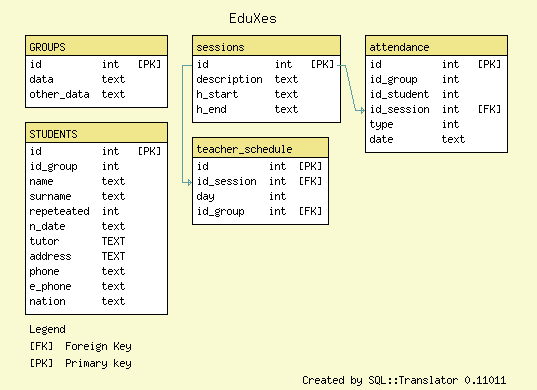
\includegraphics[width=14.208cm,height=10.319cm]{PhoneGapProjectMSWLMemory-img/PhoneGapProjectMSWLMemory-img6.png}
\caption[EduXes Database structure]{EduXes Database structure}
\label{seq:refIllustration4}

\end{figure}
\subsubsection[Preparation of development:]{Preparation of development:}
\hypertarget{RefHeading146501801272074}{}\begin{enumerate}
\item \begin{enumerate}
\item Build development environment: 

Java Development Kit (JDK) version 1.6 is downloaded from: 
\end{enumerate}
\end{enumerate}
{\itshape
http://www.oracle.com/technetwork/java/javase/downloads/index.html}

\begin{enumerate}
\item \begin{enumerate}
\item[] As root user that file is unpacked into \textit{/usr/lib/jvm}
and configured to be the Java default:
\end{enumerate}
\end{enumerate}
\textit{\# \ }\textit{update-java-alternatives -s JDK\_1.6\_NAME}

\ \ Eclipse Juno (4.6) is downloaded from its web-page:

\href{http://www.eclipse.org/}{http://www.eclipse.org}\textit{
Download-{\textgreater}Linux 64 bits}

\begin{enumerate}
\item[] Android Development Toolkit (ADT) is downloaded following
instructions on this page:
\end{enumerate}
\url{http://developer.android.com/sdk/installing/installing-adt.html}\textit{
}

\ \ A new line is included into repository software (Help \ding{213}
Install New Software \ding{213} Add):

{\itshape
http://dl-ssl.google.com/android/eclipse/}

\ \ Next step is to select all the related software listed.

\ \ For Aptana Plugin line to add into Eclipse is: 

{\itshape
http://download.aptana.com/studio3/plugin/install}

\ \ Furthermore JQuery, JQueryMobile and Phonegap are needed, and were
downloaded from their web sites:

\begin{enumerate}
\item[] JQuery 1.8.1 (no newer versions):
\end{enumerate}
\url{http://jquery.com/}\textit{ }

\begin{enumerate}
\item[] JQuery will be \ copied into \textit{assets/www/js} folder.

JQueryMobile version 1.1.1 from
\end{enumerate}
\url{http://jquerymobile.com/}\textit{ }

\begin{enumerate}
\item[] JQueryMobile is a zip file which will be uncompressed and copied
into 
\end{enumerate}
\textit{assets/www/js} folder.

\ \ PhoneGap - Cordova 1.8.1 is downloaded from this URL:

\url{https://github.com/phonegap/phonegap/zipball/1.8.1}\textit{ }

\ \ To create a PhoneGap application this very important instructions
(Getting Started with Android) \ should be followed step by step:

\url{http://docs.phonegap.com/en/1.8.1/guide_getting-started_android_index.md.html}\textit{
\ \ \ }


\bigskip

\begin{enumerate}
\item \begin{enumerate}
\item Choose application name and folder{\textquotesingle}s policy:

EduXes stands for “Educación” and “Xestión”, is a educational management
software.

A folder is created (\textit{assets/www/js}) which contains javascript
(*.js) files except JQuery and JqueryMobile which is included into
another folder (\textit{assets/www/js/jquery}), do not forget style
sheet files (*.css)
\item Make a simple application: only a blank page.

Getting started with Android is followed step by step.
\item Upload simple application into a git repository. 

A Github\footnote{\href{http://www.github.com/}{http://www.github.com} }
account is created and a new application is initialized. \ This are the
source code project page:
\end{enumerate}
\end{enumerate}
\textit{\ }\url{https://github.com/joseantoniosa/EduXes/}

\begin{enumerate}
\item \begin{enumerate}
\item[] Source code are upload to GitHub: 
\end{enumerate}
\end{enumerate}
{\itshape
\$ git init }

{\itshape
\$ git add -A *}

\textit{\$ git remote add \ EduXes
}\href{mailto:git@github.com}{git@github.com}\textit{:joseantoniosa/EduXes.git
}

{\itshape
\$ git push origin master}

\ \ Every time an update is going to be uploaded:

{\itshape
\$ git add -A *}

{\itshape
\$ git commit -m
{\textquotesingle}CHANGES\_DESCRIPTION{\textquotesingle}}

\textit{\$ git push origin master}


\bigskip

\begin{enumerate}
\item \begin{enumerate}
\item
\ JQueryMobile\footnote{\url{http://jquerymobile.com/demos/1.1.1/docs/}}
applications are structured in pages (\textcolor{black}{{\textless}div
data-role=”page”{\textgreater}}), which are very similar to desktop
applications windows, therefore, from Javascript code, to change to a
new page
\ \textcolor{black}{\ }\textcolor{black}{\ \$.mobile.changePage({\textquotedbl}\#daily\_work{\textquotedbl})}\textcolor{black}{
}\ opens \textcolor{black}{daily\_work p} page. \ 
\end{enumerate}
\end{enumerate}
\clearpage\subsubsection[Application Work{}-flow ]{Application Work-flow
}
\hypertarget{RefHeading146521801272074}{}Next illustration try to be
self-explicative. \ Beginning at \textcolor{black}{onDeviceReady()}
\ from interface.fs file. \ Inside each page several actions are
performed: e.g., open and populate database, load list of groups
(loadSchedule()), \ and user choose next step according options shown. 

{\centering \par}

\begin{figure}
\centering
 [Warning: Image ignored] % Unhandled or unsupported graphics:
%\includegraphics[width=17cm,height=24.042cm]{PhoneGapProjectMSWLMemory-img/PhoneGapProjectMSWLMemory-img7}
\caption[Application Skeleton]{Application Skeleton}
\label{seq:refIllustration5}

\end{figure}

\bigskip


\bigskip


\bigskip


\bigskip


\bigskip


\bigskip


\bigskip


\bigskip


\bigskip


\bigskip


\bigskip


\bigskip


\bigskip


\bigskip

\clearpage\subsubsection[Development:]{Development:}
\hypertarget{RefHeading146541801272074}{}\begin{enumerate}
\item[] There are two JavaScript files:

\begin{enumerate}
\item[] {}- \textit{interface.js}: It contains information and decisions
related to interface and application workflow, completely independent
from database.

{}- \textit{database.js}: It contains database related code: SELECT,
INSERT, etc. 
\end{enumerate}
There is only one HTML file:

\begin{enumerate}
\item[] \textit{index.html} only contains HTML framework, page
properties, and static content. \ 
\end{enumerate}
There are three important files which contain documentation:

\begin{enumerate}
\item[] {}- TODO.txt. List of goals to be achieved and milestone
reached.

{}- DATABASE.sql \ Data-base structure in SQL format.

{}- REAME.txt. Only contains general information about this application.
\end{enumerate}
Next step in development is populate database.

\begin{enumerate}
\item Populate database with sample data. To test application, sample
data are needed. 
\item Groups: These pages are not active.

\begin{itemize}
\item Make a list of groups window (aka “page”).
\item Make a group management window.
\end{itemize}
\item Students: These pages are not active.

\begin{itemize}
\item Make list of students window.
\item Students management window (insert-update-delete students)
\end{itemize}
\item Timetable for actual date: list of groups for selected day.
\end{enumerate}
\end{enumerate}
Below queryScheduleSuccess() and querySchedulePerDayDB() functions are
written, these functions fills \textcolor{black}{daily\_schedule} page
as shown in Illustration 6: Application Skeleton.


\bigskip

\begin{center}
\tablehead{}
\begin{supertabular}{|m{16.619999cm}|}
\hline
/*

\ * \ Main Window

\ */

function queryScheduleSuccess(tx, results) \{

\ var len = results.rows.length;

\ \ \ \$({\textquotesingle}\#groups\_day\_ul{\textquotesingle}).empty();

\ \ \ var html;

\ \ \ var id=0;

\ \ \ var description={\textquotedbl}{\textquotedbl};

\ \ \ var start = {\textquotedbl}{\textquotedbl};

\ \ \ var t\_id\_session=-1;

\ \ \ for (var i=0;i{\textless}len;i++) \{

\ \ \ \ \ id = results.rows.item(i).id;

\ \ \ \ \ t\_id\_session = results.rows.item(i).t\_id\_session;

\ \ \ \ \ start = results.rows.item(i).s\_h\_start; \ 

\ \ \ \ \ description = results.rows.item(i).description; 

\ \ \ \ \ html =
{\textquotedbl}{\textless}li{\textgreater}{\textquotedbl};

\ \ \ \ \ html += {\textquotedbl}{\textless}div
data-role={\textquotesingle}fieldcontain{\textquotesingle}{\textgreater}{\textquotedbl};

\ \ \ \ \ html += start;

\ \ html += {\textquotedbl}{\textless}a
data-role={\textquotesingle}button{\textquotesingle}
data-iconpos={\textquotesingle}notext{\textquotesingle}
style={\textquotesingle}float: right;{\textquotesingle}
href={\textquotesingle}index.html\#list\_students\_attendance{\textquotesingle}
{\textquotedbl};

\ \ \ html += {\textquotedbl}
onClick={\textbackslash}{\textquotedbl}listStudentsAttendance({\textquotedbl}
+ results.rows.item(i).t\_id\_group +
{\textquotedbl},{\textquotedbl}+t\_id\_session +
{\textquotedbl});{\textbackslash}{\textquotedbl}{\textgreater}{\textquotedbl}
+ description +
{\textquotedbl}{\textless}/a{\textgreater}{\textquotedbl};

\ \ \ \ html += {\textquotedbl}{\textquotedbl};

\ \ \ \ html +=
{\textquotedbl}{\textless}/div{\textgreater}{\textquotedbl};

\ \ \ \ html +=
{\textquotedbl}{\textless}/li{\textgreater}{\textquotedbl};

\ \ \ \$({\textquotesingle}\#groups\_day\_ul{\textquotesingle}).append(html);

\ \ \ \}

\ \ \ \$({\textquotesingle}\#groups\_day\_ul{\textquotesingle}).listview({\textquotesingle}refresh{\textquotesingle});

\ \ \ \}\\\hline
\end{supertabular}
\end{center}

\bigskip

\begin{center}
\tablehead{}
\begin{supertabular}{|m{16.619999cm}|}
\hline
/* Query groups per day - Main Window -

*/

function querySchedulePerDayDB(tx)\{

\ var query = {\textquotedbl}SELECT teacher\_schedule.id\_session,
teacher\_schedule.day, teacher\_schedule.id\_group as t\_id\_group,
teacher\_schedule.id\_session as t\_id\_session, {\textquotedbl};

\ \ query += {\textquotedbl} groups.id as g\_id, groups.data as
description, sessions.id as s\_id, sessions.h\_start as s\_h\_start,
sessions.h\_end as s\_h\_text FROM teacher\_schedule, groups, sessions
{\textquotedbl};

\ \ query += {\textquotedbl} WHERE day={\textquotedbl}
+week\_day\_global + {\textquotedbl} AND g\_id=t\_id\_group AND
t\_id\_session=s\_id \ ORDER BY t\_id\_session;{\textquotedbl};

\ \ console.log({\textquotedbl}querySchedulePerDayDB:{\textquotedbl} +
query);

\ \ tx.executeSql(query,[], dbSuccessFunc = function(tx,rs)\{

\ \ \ \ \ \ \ \ \ \ \ \ \ \ \ \ queryScheduleSuccess(tx, rs);\},

\ \ \ \ \ \ \ \ \ \ \ \ dbErrorFunc = function(tx, e) \{

\ \ \ \ \ \ \ \ \ \ \ \ \ \ \ \ if (tx.message) e = tx;

\ \ \ \ \ \ \ \ \ \ \ \ \ \ \ \ alert({\textquotedbl} There has been an
error QuerySchedulePerDayDB: {\textquotedbl} + e.message);

\ \ \ \ \ \ \ \ \ \ \ \ \ \ \ \ return false;

\ \ \ \ \ \ \ \ \ \ \ \ \}); \ \ 

\}\\\hline
\end{supertabular}
\end{center}

\bigskip

\begin{enumerate}
\item \begin{enumerate}
\item Add attendance, misbehaviour for each student. Student attendance,
misbehaviour, punctuality are set here.
\end{enumerate}
\end{enumerate}
\subsection[Tasks to be done]{Tasks to be done}
\hypertarget{RefHeading150271801272074}{}\begin{enumerate}
\item \begin{enumerate}
\item Add error handling. Error handling is managed throw dbErrorFunc.
\item Retrieve and insert data from and to database. 
\item List of attendance, misbehaviour incidents. A list of attendance
will be carried on, reusing Siestta interfaces.
\item Add activities grades for each student. 
\item List students marks and final mark. On a window, group, student
name and surname will be shown, and a table with his/her marks.
\item Activities management window. Add, remove and update activities.
It includes name of activity and percent weight.
\item Management of student notes. Student{\textquotesingle}s notes
could be included as an option.
\item List of student notes. In a table-like window, notes will be
displayed.
\end{enumerate}
\end{enumerate}

\bigskip

Next pages show several windows/pages already implemented.

\begin{enumerate}
\item \begin{enumerate}
\item[] \clearpage

\begin{figure}
\centering
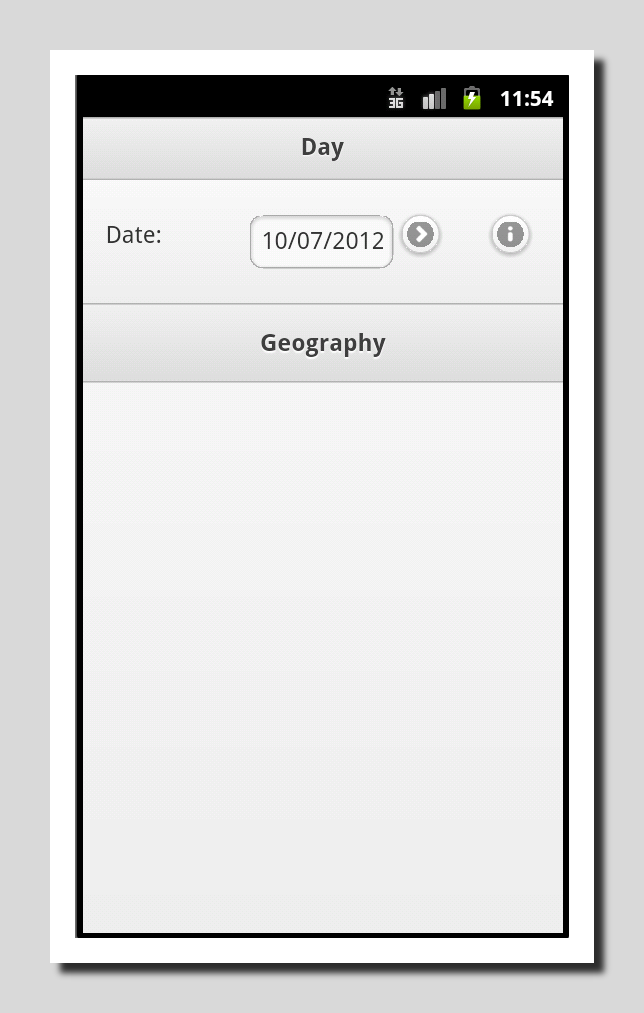
\includegraphics[width=15.73cm,height=24.742cm]{PhoneGapProjectMSWLMemory-img/PhoneGapProjectMSWLMemory-img8.png}
\caption[Main Window]{Main Window}

\end{figure}
\clearpage

\begin{figure}
\centering
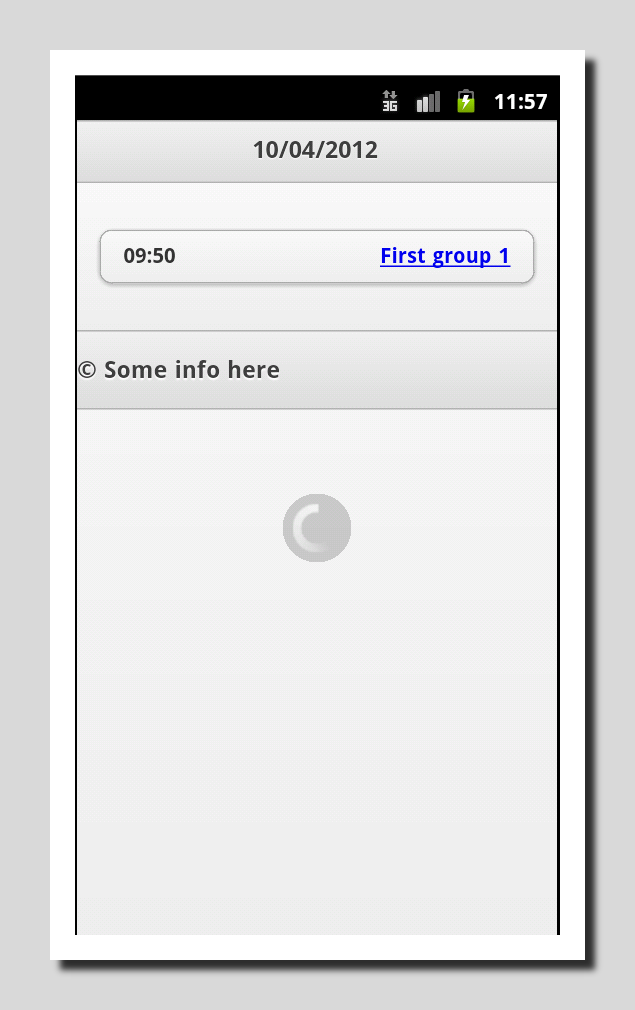
\includegraphics[width=15.73cm,height=25.019cm]{PhoneGapProjectMSWLMemory-img/PhoneGapProjectMSWLMemory-img9.png}
\caption[Classes per day.]{Classes per day.}

\end{figure}
\clearpage

\begin{figure}
\centering
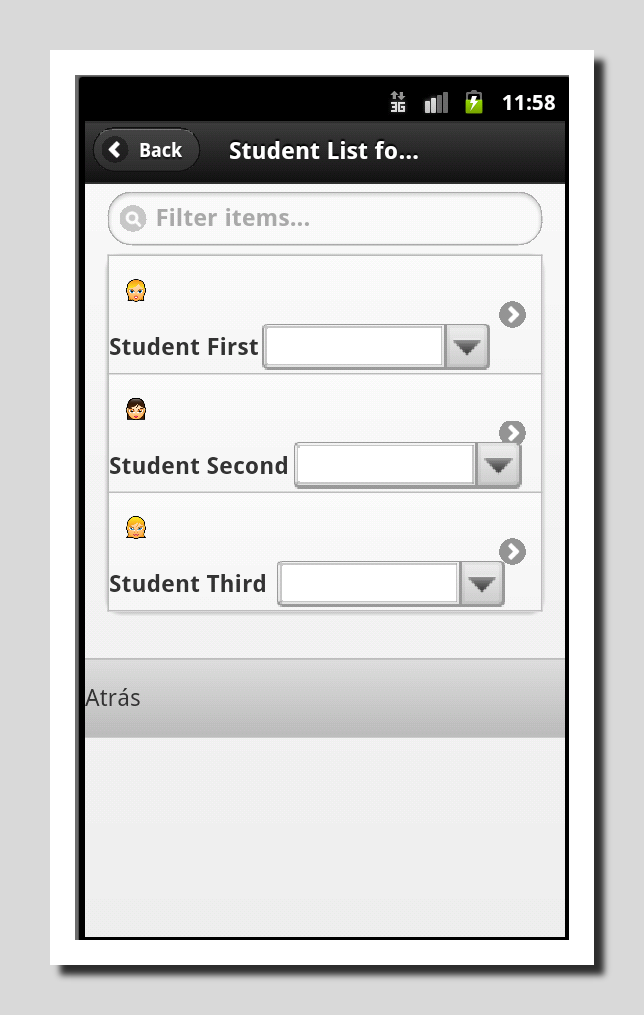
\includegraphics[width=15.73cm,height=24.791cm]{PhoneGapProjectMSWLMemory-img/PhoneGapProjectMSWLMemory-img10.png}
\caption[Students per group.]{Students per group.}

\end{figure}
\clearpage

\begin{figure}
\centering
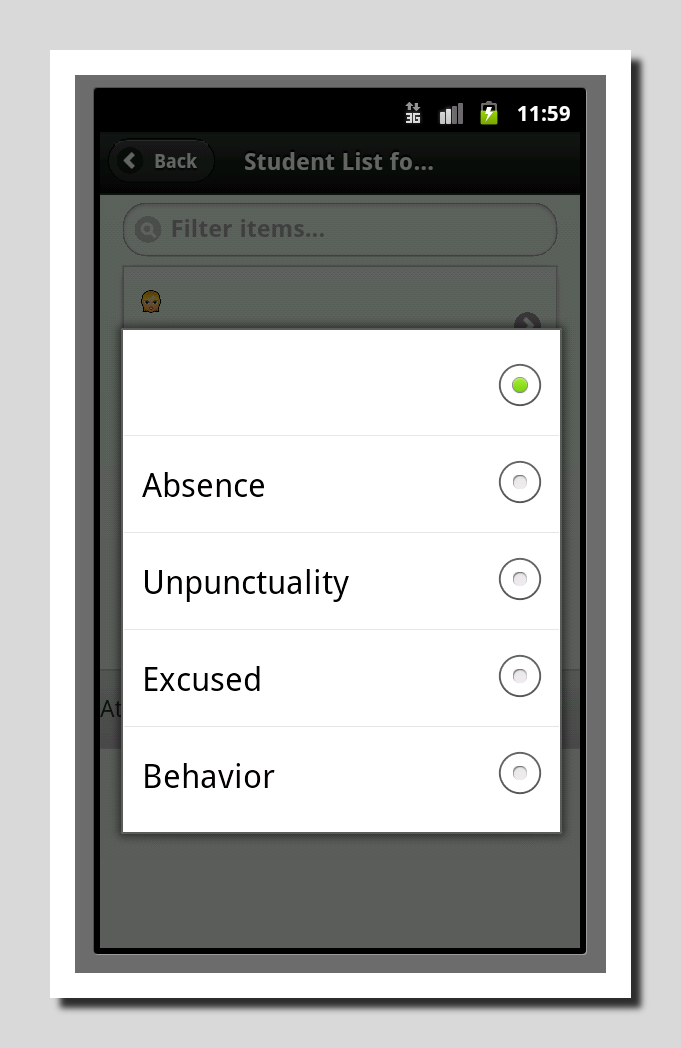
\includegraphics[width=15.73cm,height=24.208cm]{PhoneGapProjectMSWLMemory-img/PhoneGapProjectMSWLMemory-img11.png}
\caption[Student absence/unpunctuality/behaviour.]{Student
absence/unpunctuality/behaviour.}

\end{figure}
\clearpage
\bigskip
\end{enumerate}
\end{enumerate}
\subsubsection[Test into real hardware]{Test into real hardware}
\hypertarget{RefHeading146561801272074}{}\begin{enumerate}
\item[] \ Android 2.3.3 mobile phone will be used to test application.
This is not done yet. Seems to be problems copying .apk file into disk
phone.
\end{enumerate}
\subsubsection[Save or download data from database to disk]{Save or
download data from database to disk}
\hypertarget{RefHeading146581801272074}{}SQLite database should be saved
into an external
file.\footnote{\url{http://docs.phonegap.com/en/1.8.1/cordova_file_file.md.html\#File}}

\subsubsection[Xade web interface]{Xade web interface}
\hypertarget{RefHeading146601801272074}{}\begin{enumerate}
\item \begin{enumerate}
\item Study Xade web interface. Using accessibility tools Xade will be
parsed looking for information: students data, groups, etc.
\item Develop an ad-hoc application for retrieve Xade{\textquotesingle}s
data. 
\end{enumerate}
\end{enumerate}
\subsubsection[Another developments]{Another developments}
\hypertarget{RefHeading146621801272074}{}\begin{enumerate}
\item Develop an ad-hoc application for store data. This application
will be platform specific.
\item Synchronization with a custom server or with Xade. With above
information about Xade interface it could be possible to upload some
information into Xade.
\end{enumerate}
\subsubsection[Test units. ]{Test units. }
\hypertarget{RefHeading146641801272074}{}Need to be written for each
capability and function.

\subsubsection[User documentation]{User documentation}
\hypertarget{RefHeading146661801272074}{}\ Manual with images. Need to
be written with screen-shots or a screen-cast.

\subsubsection[Developer{\textquotesingle}s
documentation]{Developer{\textquotesingle}s documentation}
\hypertarget{RefHeading146681801272074}{}\ API should be documented,
application overview will be written and several diagrams will be
drawn.

\clearpage\subsubsection[Community]{Community}
\hypertarget{RefHeading146701801272074}{}Find out a site to host: forum,
bug reports, documentation and to download application
itself.\footnote{\begin{enumerate}
\item[]
\url{http://en.wikipedia.org/wiki/Comparison_of_open_source_software_hosting_facilities}
\end{enumerate}
} This is a very important milestone, because could allow to improve
application itself, and to listen users opinions. \ 

\begin{enumerate}
\item[] 
\bigskip


\bigskip
\end{enumerate}
\section[\ Personal evaluation of the practicum ]{\ Personal evaluation
of the practicum }
\hypertarget{RefHeading114201570052158}{}Firstly, it was really
difficult to prepare environment, because there a lot of
incompatibilities among plug-ins, Eclipse versions and son on, at last
I think it was my fault, I used to find out the most complicated
solutions for not-so-difficult problems. 

\ \ On the other hand, coding was effortless, despite of application
work-flow confusion and increasing complexity. My mentor, Manuel Rego
help me a lot, he told me an overview of how JQueryMobile, PhoneGap
works, and how to work step-by-step; \ I should follow his code-style
(e.g. use append function and do not work directly with strings), but I
have felt more comfortable with my old-fashioned coding-style. Of
course I have reused several SergasApp functions. 

\ \ Eventually this application could be a never ending story, really
difficult and complicated. Several functions should be rewritten.

\ \ Honestly, I am not really a good coder, nor a good graphical user
interface designer neither a good database designer. At this point I
realized that Siestta developer did a good job. I feel far away from be
a good coder, but \ it works, at least for me. \ 


\bigskip


\bigskip


\bigskip


\bigskip

\clearpage
\bigskip

Acknowledgements:

\begin{itemize}
\item To my mentor. Manuel Rego.
\item To Ramón Castro Perez who sent me a patch to allow Siestta work.
\item José Manuel Ciges Regueiro, which memory I used as a template for
my own work. \ \ \ \ \ \ \ \ \ 


\bigskip

\clearpage
\bigskip
\end{itemize}
Tools used:

\begin{itemize}
\item Sqlfairy. Tranforms SQL language into a \ png image.
\item LibreOffice 3.5.4.2 to write this document. \footnote{\ I rather
LaTeX, but LibreOffice is straightforward.} 
\item Gimp 2.8.2 to get screen-shots.
\item GNU/ Debian Wheeze October 2012 


\bigskip
\end{itemize}
References:

\begin{itemize}
\item Comparison among open source hosting facilities:
\url{http://en.wikipedia.org/wiki/Comparison_of_open_source_software_hosting_facilities}
\item W3C Database Specifications:
\url{http://www.w3.org/TR/webdatabase/}
\item PhoneGap Storage:
\ \url{http://docs.phonegap.com/en/1.8.1/cordova_storage_storage.md.html}
\item JqueryMobile: \url{http://jquerymobile.com/demos/1.1.1/}
\item Jquery: \url{http://docs.jquery.com/}
\item SergasApp: \url{http://mrego.github.com/sergasapp/}
\item EduXes: \url{https://github.com/joseantoniosa/EduXes/}
\item Siestta: \url{http://siestta.sourceforge.net/doc/index.html}
\item Xade Web: \url{https://auth.edu.xunta.es/cas/login} 
\end{itemize}

\bigskip

This document is hosted at:

\url{https://github.com/joseantoniosa/EduXes/blob/master/docs/PhoneGap_Project_MSWL_Memory.odt}
\end{document}
